\documentclass[11pt]{article}
\usepackage[toc,page]{appendix}
\usepackage{amsmath, amssymb}
\usepackage[utf8]{inputenc}
\usepackage[T1]{fontenc}
\usepackage[style=apa,backend=biber]{biblatex}
%\usepackage{biblatex}
\addbibresource{references.bib}
\usepackage{graphicx}
\usepackage{tikz}
\usetikzlibrary{automata,positioning,shapes.geometric, arrows.meta, fit, backgrounds, calc, chains}
\graphicspath{./images/Easy_Pictures/SMR_MULT_Repackaging}%\usepackage{kpfonts}
\usepackage{float}
\usepackage[margin=1in]{geometry}
\usepackage{cancel}
\usepackage{epsfig}
\usepackage{tikz-3dplot}
\usepackage{darkmode}
\usepackage{dirtytalk}
\usepackage{longtable,booktabs,array}
\usepackage{calc} % for calculating minipage widths
\usepackage[utf8]{inputenc}
\usepackage[T1]{fontenc}
\usepackage{xcolor}
\usepackage{listings}


\usepackage{etoolbox}
\usepackage{hyperref}
\hypersetup{
    colorlinks=true,
    linkcolor=blue,
    filecolor=magenta,      
    urlcolor=cyan,
    pdftitle={Hermeneutic Calculator},
    citecolor=blue,
    }


\urlstyle{same}

\lstdefinestyle{htmlStyle}{
    language=HTML,
    basicstyle=\ttfamily\small,
    keywordstyle=\color{blue}\bfseries,
    commentstyle=\color{gray}\itshape,
    stringstyle=\color{red},
    breaklines=true,
    frame=single,
    numbers=left,
    numberstyle=\tiny\color{gray},
    columns=fullflexible,
}
\lstdefinelanguage{HTML}{
  keywords={<!DOCTYPE, html, head, title, body, h1, h2, h3, p, div, span, a, img, ul, li, table, tr, td, th, style, link, script},
  sensitive=true,
  comment=[l]{//},
  morecomment=[s]{/*}{*/},
  morestring=[b]',
  morestring=[b]"
}
\lstset{style=htmlstyle, language=html}
% Updated to explicitly pass the language option
%\lstinputlisting[style=htmlstyle, language=html]{./html/example.html}
%\usepackage{tocloft}

% Optional: define some custom colors
\definecolor{sliceRed}{RGB}{225,224,91} % matching "varyellow" from your code
\definecolor{linkYellow}{RGB}{255,215,0}  % a golden yellow
\tdplotsetmaincoords{70}{110}

\title{Division Strategies - Using Commutative Reasoning}
\author{Compiled by: Theodore M. Savich}
\date{\today}

\begin{document}
\maketitle

Strategy descriptions and examples adapted from \textcite{HackenbergCourseNotes}.

This is a strategy for transforming the context of a sharing division problem (where the number of items in each group is unknown) into one where measurement division strategies can be used. Measurement division strategies are generally easier to use because students can count something. 

\bigskip

$\fbox{Number of groups} \times \fbox{Unknown Number of items in each group}  = \fbox{Total number of items}$



The idea of \textbf{Using Commutative Reasoning} is to reframe $N$ —- the number of groups -— as the act of placing one item into each group simultaneously. So, when you count one $N$, you're putting one item into every group; counting three $N$s means each group receives three items. This new interpretation of $N$ enables us to apply measurement division strategies, since our goal becomes finding how many times $N$ fits into the total number of items. This method is incredibly useful—but first, we need to clarify this shift in how we view $N$! You might create a chart that illustrates distributing items one round at a time across the groups as you count by $N$. When you're learning this strategy, using such visual representations can be very beneficial. The problem remains a sharing division problem, but we can now effectively apply measurement division strategies to solve it.


\noindent Example: There are 56 cupcakes and 8 boxes. If we are going to put an equal number of cupcakes in each box, how many will go in each box?


The original meaning of 8 in the problem is \# of boxes, or \# of
groups. The meaning Victoria gave to 8 when she wrote down eight 8s (see
above) was that 8 meant the \# of items in a group. Neither of these
meanings for 8 would allow her to count by repeatedly by 8 until she
reaches 56, and then to know she has solved the problem. In other
words, neither of these meanings for 8 will allow her to count seven 8s
as a meaningful solution to the problem. WHY?

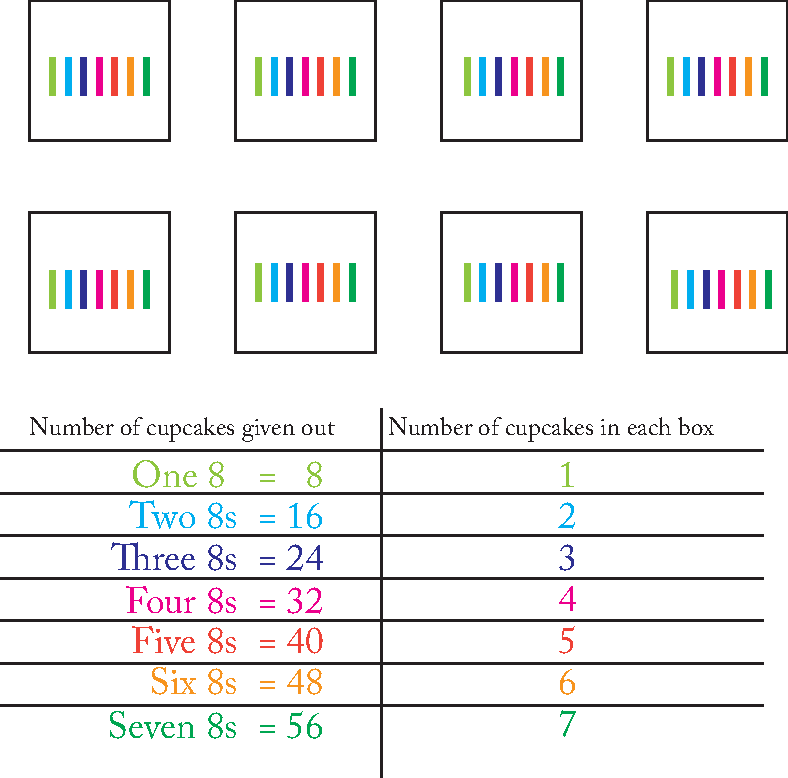
\includegraphics[width=.8\textwidth]{images/Easy_Pictures/SMR_DIV_UCR/PDF/SMR_DIV_UCR.pdf}


\subsection*{Using Commutative Reasoning}

\subsubsection*{Strategy Overview}
\textbf{Using Commutative Reasoning} leverages the commutative property of multiplication to facilitate division. By repackaging the number of groups and the number of items in each group, this strategy simplifies the division process and aligns it with multiplication reasoning.

\subsubsection*{Automaton as a 7-Tuple}
\[
M = 
\bigl(Q,\, \Sigma,\, \Gamma,\, \delta,\, q_{0},\, \#,\, F\bigr),
\]
where:
\begin{itemize}
    \item \(Q = \{\,q_{0},\; q_{\text{read}},\; q_{\text{calculate}},\; q_{\text{output}},\; q_{\text{accept}}\}\).
    \item \(\Sigma = \{G, E\}\) is the input alphabet 
          (\(G\) = group information, \(E\) = total items).
    \item \(\Gamma = \{\#,\, G,\, E,\, Q\}\) is the stack alphabet, with \(\#\) the bottom marker.
    \item \(q_{0}\) is the start state; 
    \item \(\#\) is the initial stack symbol.
    \item \(F = \{\,q_{\text{accept}}\}\) is the set of accepting states.
\end{itemize}

\subsubsection*{State Transition Table (Corrected)}
\begin{center}
\renewcommand{\arraystretch}{1.3}
\begin{tabular}{|c|c|c|c|c|p{4.8cm}|}
\hline
\textbf{Current} & \textbf{Input} & \textbf{Stack} & \textbf{Next} & 
\textbf{Stack} & \textbf{Action /}\\
\textbf{State} & \textbf{Symbol} & \textbf{Top}   & \textbf{State} & 
\textbf{Operation} & \textbf{Interpretation}\\
\hline
\(q_{0}\) & \(\varepsilon\) & (empty) & \(q_{\text{read}}\) & Push \(\#\) & 
Initialize stack with \(\#\).\\
\hline
\(q_{\text{read}}\) & \(G\) & \(\#\) & \(q_{\text{read}}\) & Push \(G\) & 
Read group info.\\
\hline
\(q_{\text{read}}\) & \(E\) & \(G\) & \(q_{\text{calculate}}\) & Push \(E\) & 
Read total elements.\\
\hline
\(q_{\text{calculate}}\) & \(\varepsilon\) & \(E\) & \(q_{\text{output}}\) & 
Pop \(E\), Pop \(G\), Push \(Q=E/G\) & 
Perform division \(E \div G\).\\
\hline
\(q_{\text{output}}\) & \(\varepsilon\) & \(Q\) & \(q_{\text{accept}}\) & 
Output \(Q\) & Show result (quotient).\\
\hline
\(q_{\text{accept}}\) & \(\varepsilon\) & \(\#\) & \(q_{\text{accept}}\) & 
No change & Accept.\\
\hline
\end{tabular}
\end{center}

\subsubsection*{Automaton Behavior (Step-by-Step)}
\begin{enumerate}
  \item \textbf{Initialization:} In state \(q_{0}\), push the bottom‐of‐stack marker \(\#\), then move to \(q_{\text{read}}\).
  \item \textbf{Reading the Inputs:} 
    \begin{itemize}
      \item Reading \(G\) (e.g.\ 8): push \(G\) onto the stack.
      \item Reading \(E\) (e.g.\ 56): push \(E\) onto the stack, then move to \(q_{\text{calculate}}\).
    \end{itemize}
  \item \textbf{Calculation:} In \(q_{\text{calculate}}\), pop both \(E\) and \(G\), compute the quotient \(Q = \tfrac{E}{G}\), and push \(Q\). 
  \item \textbf{Output:} Transition to \(q_{\text{output}}\), output \(Q\), then move to \(q_{\text{accept}}\) to finish.
\end{enumerate}

\subsubsection*{Corrected Example Execution}
\[
\text{Problem: Divide } 56 \text{ items into } 8 \text{ groups.}
\]
\begin{enumerate}
  \item \textbf{Inputs Read:}
    \[
      G = 8,\quad E = 56.
    \]
  \item \textbf{Stored on Stack:} \(\#\) at the bottom, then \(G\), then \(E\).
  \item \textbf{Calculation Step:} 
    \[
      Q = \frac{E}{G} = \frac{56}{8} = 7.
    \]
  \item \textbf{Output:} The automaton pushes \(Q=7\) and transitions to \(q_{\text{output}}\).  
\end{enumerate}
No contradictory “\(\tfrac{8}{56}\)” arises here, because we never literally swap the roles of \(G\) and \(E\). Instead, the “commutative” viewpoint is *conceptual*: we regard “8 groups” as “counting by eights” out of 56, which is the usual measurement‐division approach.

\bigskip


\clearpage

\subsubsection*{HTML Implementation}
%\lstinputlisting[style=htmlStyle, language=html]{./new_html/}

\printbibliography

\end{document}